\begin{figure}[H]
    \centering
    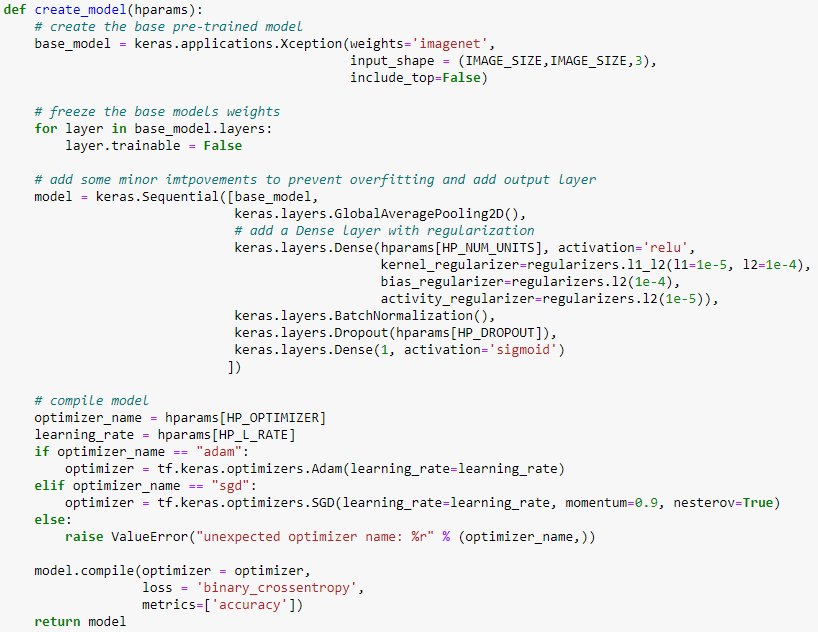
\includegraphics[width=\textwidth]{figures/xception-improvement-1.png}
    \caption{Freezing the base models trainable weights.}
    \label{fig:xception-improvement-1}
\end{figure}
\begin{figure}[H]
    \centering
    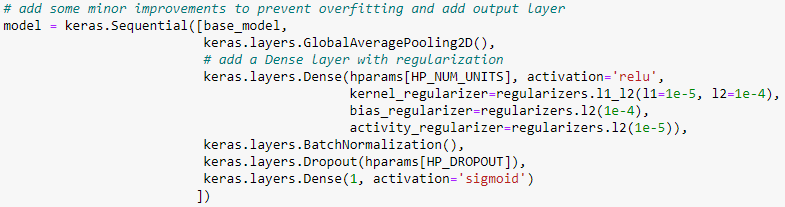
\includegraphics[width=\textwidth]{figures/xception-improvement-2.png}
    \caption{Adding regularisers to the Dense layer.}
    \label{fig:xception-improvement-2}
\end{figure}
\begin{figure}[H]
    \centering
    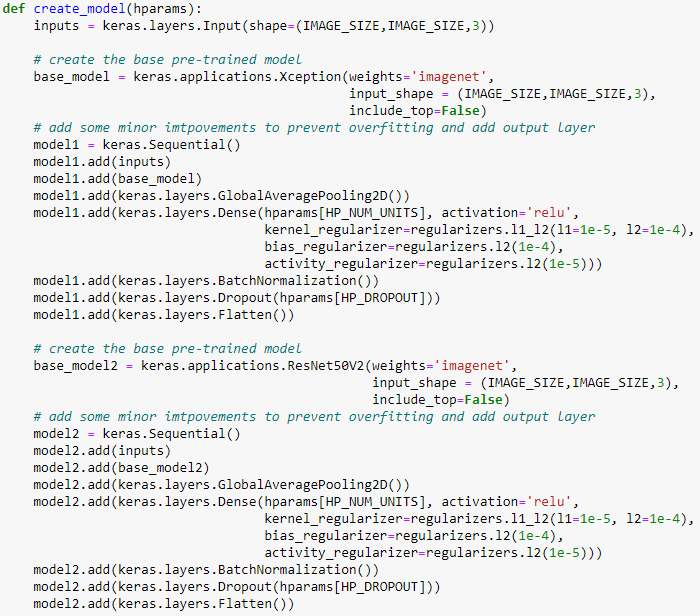
\includegraphics[width=\textwidth]{figures/xception-improvement-3-part1.png}
    \caption{The first half of the Xception-ResNet50V2 model.}
    \label{fig:xception-improvement-3-part1}
\end{figure}
\begin{figure}[H]
    \centering
    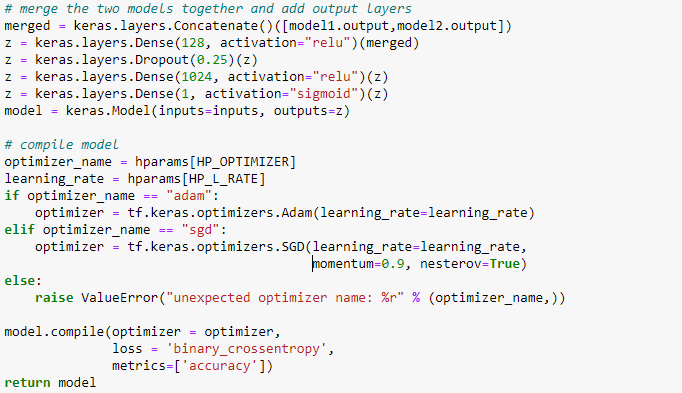
\includegraphics[width=\textwidth]{figures/xception-improvement-3-part2.png}
    \caption{The second half of the Xception-ResNet50V2 model.}
    \label{fig:xception-improvement-3-part2}
\end{figure}
\begin{figure}[H]
    \centering
    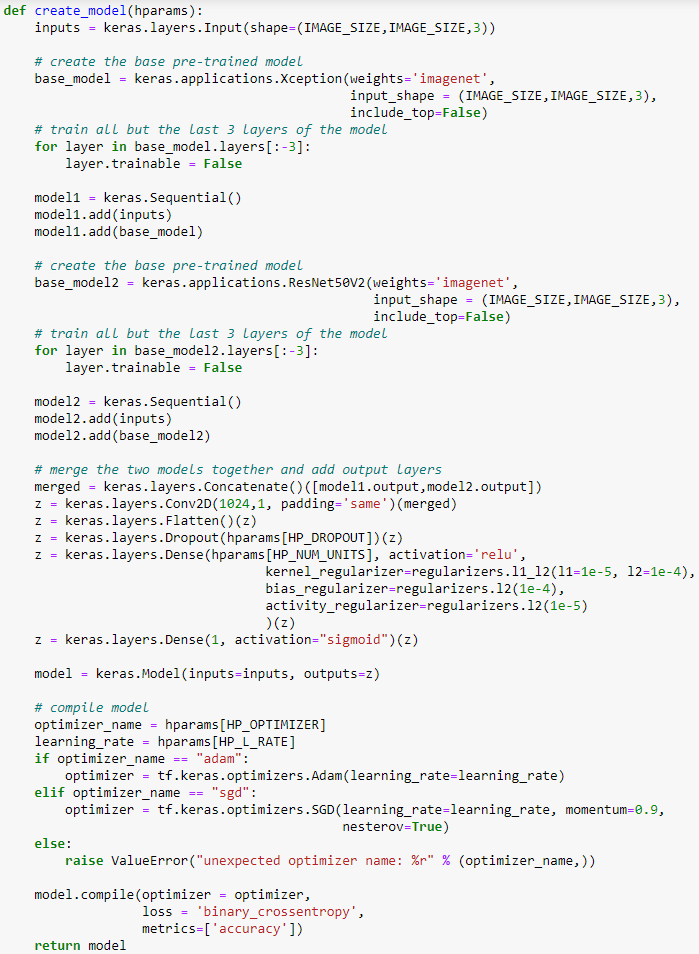
\includegraphics[width=\textwidth]{figures/xception-improvement-4.png}
    \caption{The second version of the Xception-ResNet50V2 model.}
    \label{fig:xception-improvement-4}
\end{figure}
\begin{figure}[H]
    \centering
    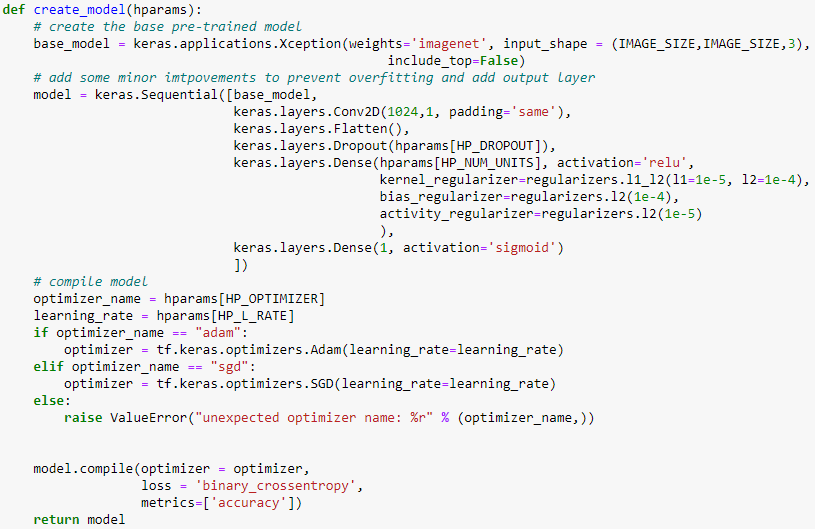
\includegraphics[width=\textwidth]{figures/xception-improvement-5.png}
    \caption{The final improvement to the Xception model.}
    \label{fig:xception-improvement-5}
\end{figure}